	\section{\ttZ Production Details}
	The production of a top-antitop pair in association with a Z boson primarily occurs with two types of diagrams at Leading Order (LO). One diagram is a combination of the two standard diagrams for \ttbar production and Z production from quark-antiquark interactions. It is more rare than either of those productions on their own (which have been well measured) because it relies on both vertices being present with multiple quark interactions. The second production is somewhat more interesting because it is a process that has never been measured before. This production involves the unmeasured EWK coupling of the Z boson to a top and is best understood as a radiative interaction by top particles with very high momentum. See Fig~\ref{fig:ttz_LO_diagrams} for the Feynman diagrams of these two LO processes.\\
	\begin{figure}[h]
\begin{center}
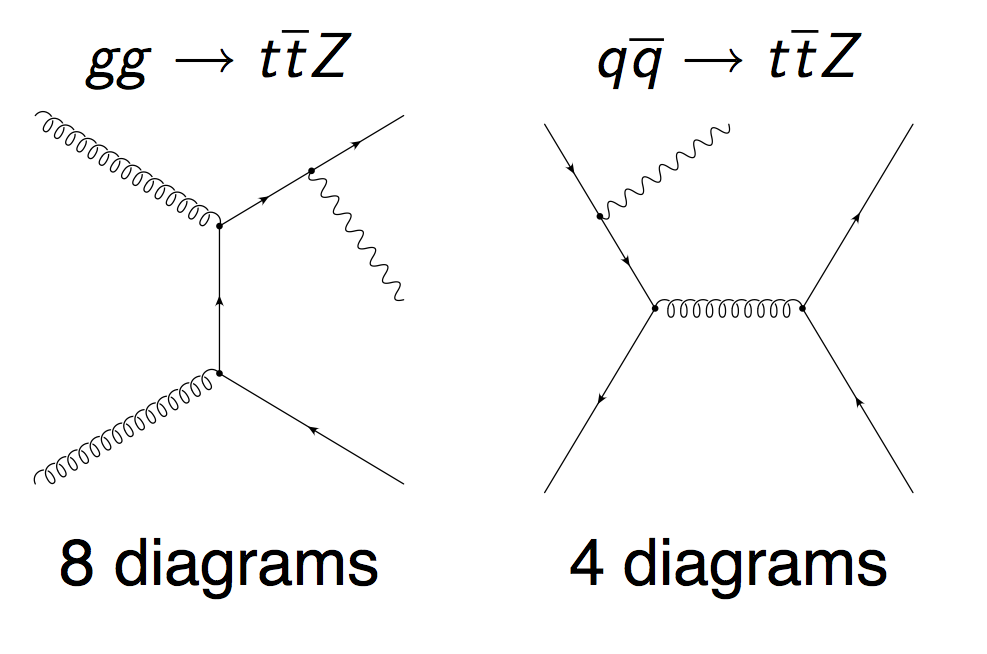
\includegraphics[width=0.7\linewidth]{Figs/ttz_LO_diagrams.png}
\caption{\label{fig:ttz_LO_diagrams}
 Feynman diagrams of the Leading Order (LO) diagrams for ttZ and multiplicities of the diagrams. In the gluon produced diagrams (Left), it is best to think of the Z as a radiative process off of the top. In the quark produced diagrams (Right), the Z production is best thought of as quark annihilation.
}
\end{center}
\end{figure}

	\ttZ production is interesting both as a background for more exotic productions (like SUSY) and also as a confirmation of Standard Model predictions. The EWK coupling of the Z to the top has not been measured yet. A measurement with the coupling consistent with the SM prediction will help to rule out certain BSM models while a measurement not consistent with the SM prediction would give very important clues to new sectors of particle physics. Measuring the \ttZ cross section is a first step towards measuring this coupling constant. More data, though, will be needed than in the topic of this dissertation to measure the coupling constant of the Z to the top independently.\\
	
	\section{\ttZ Decay Details}
	After the hard collision, three objects exist that will be indirectly studied: a top, an anti-top, and a Z boson. For all intents and purposes, the top and anti-top particles behave similarly just swapping the matter and anti-matter labels in the decay products. A top quark is very massive at $\sim$173 \GeV of energy and thus decays very quickly. There is no time for it to decay via the strong force and to hadronize, so it does not form jets. The top quark can only decay to a W boson plus a down-type quark which is a b-quark the vast majority of the time. \\
	
	The b-quarks from the top and anti-top will hadronize and form b-jets which can be reconstructed with varying degrees of efficiency and purity (see Sec~\ref{sec:bTagSelection}) and act as markers for top events as high quality b-tags are fairly fair except in top or boson decays. The W and Z bosons will decay either to hadronic or leptonic final states. The W decays to either a lepton and a neutrino ($\sim$11\% per lepton flavor~\cite{pdg}) or to an up-type quark and a down-type quark (weakly). For the Z boson, quark anti-quark pairs are common (the most being \bbbar pairs which decay contributes to the \ttZ backgrounds) and also to lepton anti-lepton pairs ($\sim$ 3.3\% per lepton flavor~\cite{pdg}).\\
	
	Thus several final states exist:
	\begin{enumerate}
	\item 8 quarks (at least 2 of which are b-quarks)
	\item 6 quarks (at least 2 of which are b-quarks), 1 lepton, and 1 neutrino
	\item 6 quarks (at least 2 of which are b-quarks) and 2 leptons
	\item 4 quarks (at least 2 of which are b-quarks), 2 leptons, and 2 neutrinos
	\item 4 quarks (at least 2 of which are b-quarks), 3 leptons, and 1 neutrino
	\item 2 b-quarks, 4 leptons, and 2 neutrinos
	\end{enumerate}
	
	Thus there are several different signatures to look for in order to identify a \ttZ decay. As shown in Fig~\ref{fig:ttZ_decay_rates}, hadronic decays of the bosons are more common, with the states containing more quarks to being more common and conversely the states with more leptons are less common. However, the rate of decay must be balanced agains how unique and easy to distinguish (measure and reconstruct its elements in the detector) from the background processes.
	
	\begin{figure}[h]
\begin{center}
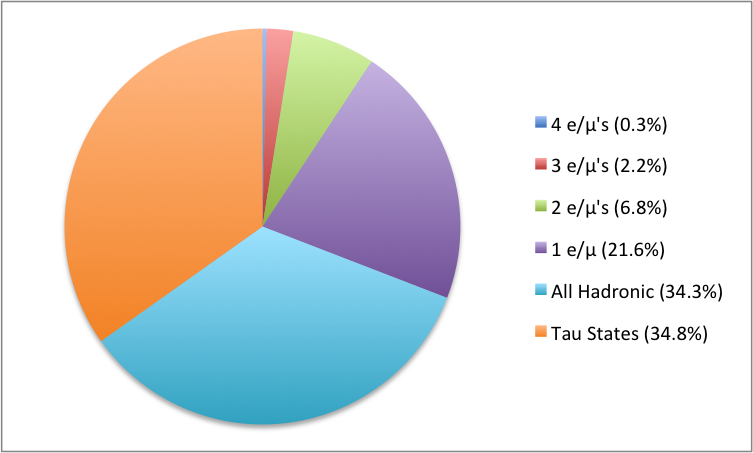
\includegraphics[width=0.8\linewidth]{Figs/ttZ_decay_fraction.png}
\caption{\label{fig:ttZ_decay_rates}
Possibly need to update this picture. Fraction of time \ttZ decays to various final states. States that contain tau decays have been separated from the states containing only electrons and muons because the measurement in this document only targets states with electrons and muons from boson decays. Decay fractions are from the Particle Data Group~\cite{pdg}.
}
\end{center}
\end{figure} 

	
	\section{Motivation for Measurement of the 3 Lepton Final State}
	In order to measure the \ttZ cross section, the final state of four quarks (at least two of which are b-quarks), three leptons, and one neutrino was chosen. This system has the advantage of several distinguishing features which make up for its lower rate of production. two of the leptons come from a Z decay and thus a mass constraint around the nominal Z mass of \zmass \ can be used to remove events with two leptons from events without a Z. The third lepton creates a rarer final state because it is unusual for a single lepton to be produced except in W decays, and there is no decay that produces three leptons from one decay. All of the states benefit from the presence of b-quarks which come from the top decay because this provides a handle to help eliminate some of the dominant backgrounds like WZ production.\\
	
	The electrons provide added bonuses in that their energy and momentum can be measured with a very high precision compared to jets, so they can be used to fairly accurately reconstruct masses such as the Z mass and the W \mt. Reconstructing these masses and showing a familiar distribution helps to bolster the claim of a \ttZ discovery. 